\begin{figure}
	\centering
	
	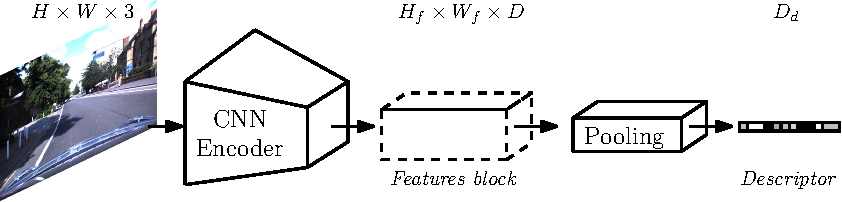
\includegraphics[width=\linewidth]{related_work/learned_desc}
	
	\caption[\acs{cnn} image descriptor]{\label{fig:cnn_aggregation} \textbf{\acs{cnn} image descriptor:} modern learned descriptors are composed of two parts: a features extractor (encoder) and a descriptor pooling method. The features block has a lower spatial resolution that the input ($W\times H > W_f\times H_f$) with more channels ($D \gg 3$). The pooling method aims to reduce the size of the features block ($D_d \ll W_f\times H_f\times D$) while keeping discriminative clues.}	
	
\end{figure}